\chapter{Metodologia} \label{metodologia}

A metodologia para desenvolver o compilador proposto envolve uma abordagem prática. As suas principais etapas são: uma análise das informações pertinentes a BRDFs e compilação de \textit{shaders}; a exploração de técnicas existentes dentro do domínio; a especificação da linguagem subconjunto \LaTeX{} de entrada;  a implementação do compilador; a avaliação de seu desempenho por meio de experimentos de renderização.

Inicialmente, o método para realizar a análise e exploração das técnicas é descrito na \autoref{analise}. Em seguida, a especificação da linguagem de entrada e saída é definida na \autoref{especificacao-linguagem} @@@{link the grammar and explain}. Posteriormente, uma ideia de como o \textit{design} dos casos de teste devem ser elaborados para validar a correção e precisão do compilador é apresentado na \autoref{testes}. O método de implementação do compilador é detalhado na \autoref{compiladorimplementacao}. A \autoref{experimentos-renderizacao} planeja o método de avaliação dos experimentos de renderização quanto a qualidade visual dos \textit{shaders} compilados. Por fim, um plano de continuação é delineado, abordando as próximas etapas para completar o desenvolvimento do compilador proposto (\autoref{continuacao}).
Seguindo essa metodologia, a ferramenta proposta visa compilar efetivamente descrições de BRDF em \textit{shaders} GLSL.


\section{Análise e Técnicas} \label{analise}




O primeiro passo envolve a realização de uma análise detalhada das áreas relacionadas ao desenvolvimento da ferramenta proposta. Isso inclui a revisão da literatura (\autoref{revisao}) sobre BRDFs, linguagens de \textit{shaders}, \textit{design} de compiladores e técnicas de renderização gráfica. Além disso, envolve o estudo de ferramentas e bibliotecas pertinentes. Durante essa análise, foram estudados conceitos de radiometria para compreender tecnicamente as BRDFs. A principal fonte de informação sobre radiância e BRDFs foi o livro ``Physically Based Rendering: From Theory To Implementation'' \cite{pbr}. Esse livro foi importante para compreensão da equação de renderização (\autoref{eq-rendering-equation}). A leitura de exemplos práticos e leitura das código fonte da ferramente \autoref{fig-disney-tool} permitiu a familiarização com o desenvolvimento de BRDFs, fornecendo uma base sólida para a compreensão do mapeamento da equação para código, aspecto fundamental para o desenvolvimento do compilador proposto neste trabalho.@

Ademais, foram exploradas diversas técnicas para compilação, como o método de Pratt \textit{Parsing} para a construção de um compilador, conforme detalhado na \autoref{parser}, somado ao uso do conhecimento de recursividade e caminhada em arvóres para realizar a analise semantica e geração de código.


\section{Especificação da Linguagem}\label{especificacao-linguagem}

As especificações da linguagem de entrada e saída para o compilador são definidas. A linguagem de entrada é uma versão simplificada do \LaTeX{}, na qual as expressões matemáticas nos ambientes \texttt{equation} são suficientes para descrever BRDFs. O \LaTeX{}  é um sistema de composição amplamente utilizado para documentos matemáticos e científicos. O ambiente \texttt{equation} é especificamente projetado para exibir equações individuais. O \autoref{equation-latex} é um exemplo de código-fonte \LaTeX{}  usando o ambiente \texttt{equation}.


\begin{codigo}[H]
\caption{\small Código-fonte de função quadrática.}
\label{equation-latex}
\begin{lstlisting}
\begin{equation}
    g(x) = ax^2 + bx + c
\end{equation}
\end{lstlisting}
\end{codigo}




Este código representa a equação quadrática \( g(x) = ax^2 + bx + c \), onde \( a \), \( b \) e \( c \) são coeficientes. O código GLSL correspondente gerado a partir dessa equação pode ser o \autoref{cod-glsl-g}.

\begin{codigo}[H]
\caption{\small Código GLSL da função quadrática g.}
\label{cod-glsl-g}
\begin{lstlisting}
float g(float x, float a, float b, float c) {
    return a * x * x + b * x + c;
}
\end{lstlisting}
\end{codigo}

@@@
O ambiente de equações \LaTeX{} é amplo demais para o projeto, entre todas os as construções matemáticas representaveis por esse ambiente um subconjunto essencial para BRDFs deve ser escolhido. Ao analisar as principais BRDFs, como os ditos em \autoref{testes}, nota-se algumas contruções indispensaveis, essas devem ser reconhecidas e entendidas o suficiente para emitir código GLSL pelo nosso 
compilador, essas são enumeradas à seguir:

\label{subconjunto-latex-equantion} \begin{enumerate}
  \item principais funções trigonometricas \verb" \tan, \sin, \cos, \arctan, \arcsin, \arccos";

\item funcão raiz quadrada \verb"\sqrt" $\left(\sqrt{}\right)$;
\item funcão exponencial \verb"\sqrt" $\left(\sqrt{}\right)$;
\item funções utilitárias como $\max, \min$, ($\max, \min$);
\item definição de equações, por exemplo \verb"f = x" (rederizado fica $f = x$).
\item denifição de funções, por exemplo  \verb"f(x, y) = x^y" (rederizado fica $f(x, y) = x^y$) respectivamente;
\item constantes comuns como \verb"\pi" ($\pi$), \verb"\epsilon" ($\epsilon$);
\item constantes especificar \verb"\theta" ($\theta$), entre outros detalhados na @ref capitulo@;
\item indicador de vetor como \verb"\vec{}" (ex: $\vec{n}$);
\item identificadores aninhandos como \verb"f_{n_{i}}" ($f_{n_{i}}$).;
\item chamada de funções \verb"f(x+y)";
\item operadores de produto vetorial (\verb"x \times y", $x \times v$), soma ($+$), multiplicação ($x*y$ ou \verb"x \cdot y", $x \cdot y$), fração (\verb"\frac{x}{y}", $\frac{x}{y}$), divisão (\verb"{x}/{y}", ${x}/{y}$), power \verb"^", ($x^y$);

\end{enumerate}

Uma descrição completa dos simbolos reconhecidos são dados no @Desenvolvimento capitulo Lexer@. Construção completa da gramatica reconhecida pelo compilador é dado em @Capitulo Desenvolvimento Parser@. Note que do potno de vista do parser e lexer alguns simbolos são apenas reconhcidos, é citado que o compilador também precisa entenderlo, e para é preciso atribuir significado especifico à esses simbolos e construções, por exemplo $\omega_o$, que o angulo de saída da luz @@@ ou $f$ que é a brdf. Essa atribuição é feita em etapa de analise semantica, que vem após o parsing @ref@.

%
%
\section{Design de Casos de Teste} \label{testes}
%
%
Os casos de teste são essenciais para validar a precisão e correção do processo de tradução do compilador. Eles estabelecem uma correspondência entre as equações \LaTeX{} de entrada, que descrevem as BRDFs, e o código de \textit{shader} GLSL esperado como saída. Um exemplo específico que demonstra a eficácia do compilador pode ser construído com a BRDF de Cook-Torrance. Sua função, \texttt{cook\_torrance}, é representada pela \autoref{eq-cook-torrance} (seu código-fonte está definido no \autoref{cod-input-latex}), onde \(D\) é a função de distribuição normal, \(G\) é a função de sombreamento geométrico e \(F\) é a função de Fresnel.

Embora as funções \(D\), \(G\), \(F\) não tenham sido definidas explicitamente, é importante ressaltar que, caso essas funções fossem definidas na equação \LaTeX{}, elas também devem ser definidas no \autoref{cod-glsl-esperado}, GLSL esperado de saída. Vale resaltar que nessa sessão de metodologia estamos dandos uma versão simplificada  de como o design de casos de teste ocorre para auxiliar entendimento. Na prática, unidades, como $\rho_d$, e funções, como $D,G$ e $F$, devem estar definidas. Casos de teste completos estão disponiveis no \autoref{resultados}.


Além disso, algumas variáveis, como a normal representada por \( n \), seriam passadas como entrada no \textit{shader} de fragmentos ou declaradas como variáveis uniformes, portanto não estão definidas explicitamente na função \texttt{cook\_torrance} no \autoref{cod-glsl-esperado}; elas são variáveis implícitas. Todas as variáveis implicitas se encontram na \autoref{tabela-variaveis}. Inicialmente, o foco é definir casos de teste para avaliar apenas a geração das operações e precedências. No entanto, é importante considerar que, posteriormente, o GLSL não deverá apenas gerar a função BRDF, mas sim o \textit{shader} completo, incluindo as variáveis uniformes e a passagem da cor calculada para as próximas etapas do \textit{pipeline} gráfico.


\begin{equation} \label{eq-cook-torrance}
  \text{cook\_torrance}(\omega_i, \omega_o) = \frac{D(h)F(\omega_i, h)G(\omega_i, \omega_o, h)}{4(\omega_i \cdot n)(\omega_o \cdot n)}
\end{equation}


\begin{codigo}[H]
\caption{\small Entrada em \LaTeX\  (Cook-Torrance BRDF).}
\label{cod-input-latex}
\begin{lstlisting}
  \text{cook\_torrance}(\omega_i, \omega_o)
      = \frac{D(h)F(\omega_i, h)G(\omega_i, \omega_o, h)}{4(\omega_i \cdot n)(\omega_o \cdot n)}
\end{lstlisting}
\end{codigo}


\begin{codigo}[H]
\caption{\small Saída em GLSL esperada (Cook-Torrance BRDF).}
\label{cod-glsl-esperado}
\begin{lstlisting}[language=C]
vec3 cook_torrance(vec3 wi, vec3 wo) {
    float D_RESULT = D(h);
    vec3  F_RESULT = F(wi, wo);
    float G_RESULT = G(wi, wo, h);
    float denominador = 4.0 * dot(n, wi) * dot(n, wo);
    return D_RESULT * F_RESULT * G_RESULT / denominador;
}
\end{lstlisting}
\end{codigo}


\section{Implementação do Compilador} \label{compiladorimplementacao}
% \begin{enumerate}
%
% Definir símbolos pré-definidos como constantes matemáticas e outras quantidades.
% Implementar o processo de geração de código GLSL.
%
% Expandir os casos de teste para cobrir uma ampla gama de BRDFs. Testar o código gerado quanto à correção, tanto em código quanto em visualização e corrigir se necessário.


Este trabalho envolve várias tarefas-chave destinadas a completar o desenvolvimento do compilador proposto para converter equações \LaTeX{}  que descrevem BRDFs em código de \textit{shader} GLSL. As tarefas incluem: Criar um \textit{lexer} e \textit{parser} para aceitar equações \LaTeX{}; testar o \textit{lexer} para garantir o reconhecimento correto dos \textit{tokens}; testar o \textit{parser} para garantir que a árvore sintática está com precedência correta; definir símbolos predefinidos e constantes matemáticas; implementar o processo de geração de código GLSL usando a árvore sintática com o padrão de \textit{design} visitante (\textit{Visitor}); definir os casos de teste para cobrir uma certa variedade de BRDFs; testar o código gerado quanto à correção, incluindo as visualizações das BRDFs em algumas cenas.

A implementação do compilador é realizada utilizando a linguagem de programação Odin, conhecida por ser uma linguagem de propósito geral com foco em programação orientada a dados. Sua escolha se deve à sua capacidade de oferecer controle de baixo nível e a sua adequação para o desenvolvimento de sistemas complexos. Além disso, nenhuma biblioteca externa foi utilizada, sendo usada apenas as bibliotecas padrões básicas que acompanham a instalação da linguagem.

Técnicas de análise recursiva são utilizadas, especificamente o Pratt \textit{Parsing}. Inicialmente, o \textit{lexer} e o \textit{parser} foram implementados para o subconjunto (\autoref{subconjunto-latex-equantion}) linguagem \LaTeX{} comentado em \autoref{}. Para garantir que os fundamentos do compilador estejam funcionais, considerando precedência totalmente testada para a árvore sintática, foram criados o pacote walker, que abstrai uma maneira de andar pela AST e valida algo, esse é usado para duas coisas, uma é para adicionar parenteses expoicitando a ordem de operação, outro é recursivamente inferir os tipos de cada expressão (nós que representam valores) presentes na AST. Também, é necessario cirar um passagem de analisise semantica, pacote chamado de "checker" onde iremos anotar a AST com todos os campos relevantes como tipos (função com seu dominio e contradominio, vetor real e sua dimensão, ou número $\in \mathbb{R} $). Por ultimo, já com o AST anotadas com outras informaçoes, realizamos através do pacote "emitter" a geração de cógido glsl, pronto para ser carregado e redenrizado pela ferramenta \autoref{disney-brdf-tool}.

\section{Experimentos de Renderização} \label{experimentos-renderizacao}


Por fim, experimentos de renderização são realizados usando os \textit{shaders} gerados pelo compilador. Isso permite a avaliação do desempenho e da qualidade visual das imagens renderizadas produzidas pelos \textit{shaders} compilados. A plataforma escolhida para os testes é a ferramenta \label{disney-brdf-tool} Disney BRDF \footnote{\url{https://github.com/wdas/brdf}}, compilada localmente para modificar e adicionar outros
\textit{shaders}.


Essa ferramenta é composta por um renderizador e uma interface que permite ajustar parâmetros de BRDFs através de controles deslizantes em tempo real, fornecendo uma visualização interativa do efeito das mudanças nos parâmetros que afetam a aparência do objeto renderizado, como ilustrado na \autoref{fig-disney-tool}. O código que informa à ferramenta qual a BRDF a ser renderizada e seus possíveis parâmetros pode ser visto na \autoref{fig-disney-code}. Esse código possui um formato específico, onde se encontram algumas seções. Existe a seção para código GLSL e outra seção delimitada por \texttt{::begin parameters} e \texttt{::end parameters}, na qual podemos definir os parâmetros que se tornam constantes dessa BRDF. O nosso compilador gera shaders nesse formato.



\begin{figure}[htb]
        \caption{\label{fig-disney-tool} \small Ferramenta de visualização de BRDFs da Disney.}
        \begin{center}
            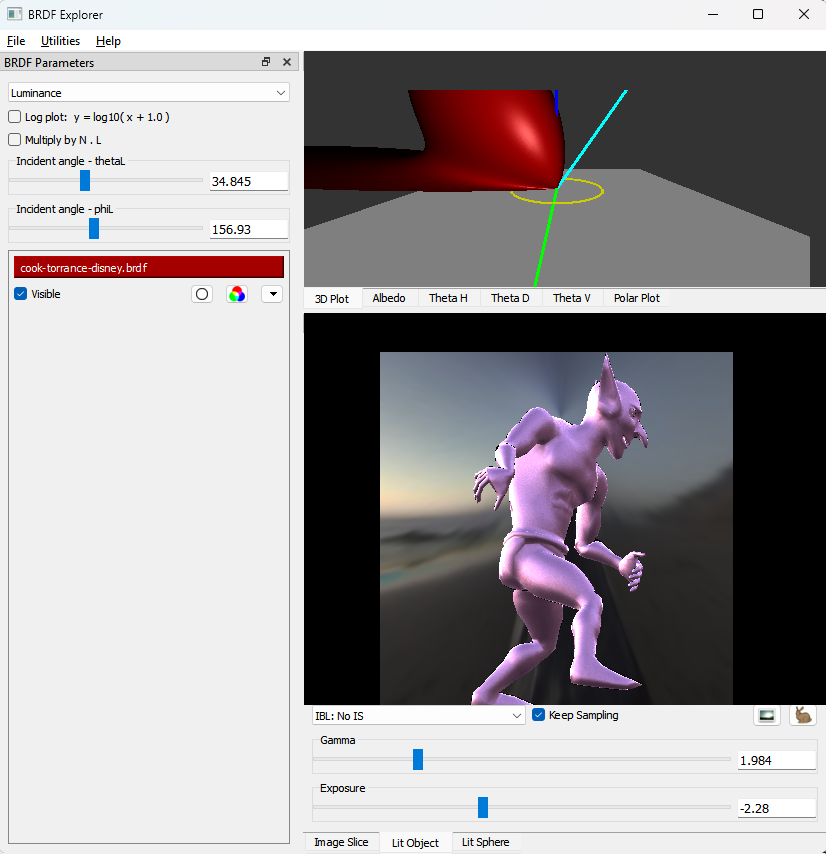
\includegraphics[scale=0.65]{./Imagens/disney-brdf-tool-original.png}
        \end{center}
  \legend{ \small Fonte: autor.}
\end{figure}


\begin{figure}[h]
        \caption{\label{fig-disney-code} \small O código GLSL com sintaxe extra para definir parâmetros.}
        \begin{center}
            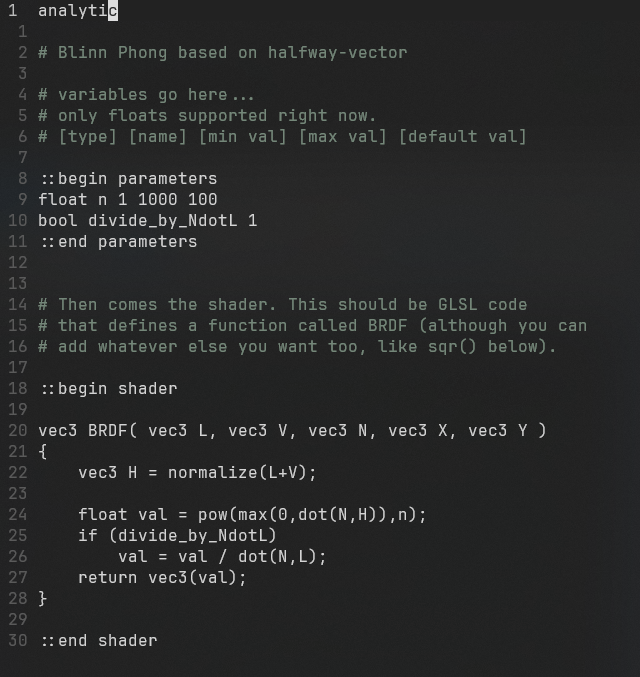
\includegraphics[scale=0.7]{./Imagens/disney-brdf-code.png}
        \end{center}
\end{figure}


